% Options for packages loaded elsewhere
\PassOptionsToPackage{unicode}{hyperref}
\PassOptionsToPackage{hyphens}{url}
%
\documentclass[
  12pt,
]{article}
\usepackage{amsmath,amssymb}
\usepackage{lmodern}
\usepackage{setspace}
\usepackage{iftex}
\ifPDFTeX
  \usepackage[T1]{fontenc}
  \usepackage[utf8]{inputenc}
  \usepackage{textcomp} % provide euro and other symbols
\else % if luatex or xetex
  \usepackage{unicode-math}
  \defaultfontfeatures{Scale=MatchLowercase}
  \defaultfontfeatures[\rmfamily]{Ligatures=TeX,Scale=1}
\fi
% Use upquote if available, for straight quotes in verbatim environments
\IfFileExists{upquote.sty}{\usepackage{upquote}}{}
\IfFileExists{microtype.sty}{% use microtype if available
  \usepackage[]{microtype}
  \UseMicrotypeSet[protrusion]{basicmath} % disable protrusion for tt fonts
}{}
\makeatletter
\@ifundefined{KOMAClassName}{% if non-KOMA class
  \IfFileExists{parskip.sty}{%
    \usepackage{parskip}
  }{% else
    \setlength{\parindent}{0pt}
    \setlength{\parskip}{6pt plus 2pt minus 1pt}}
}{% if KOMA class
  \KOMAoptions{parskip=half}}
\makeatother
\usepackage{xcolor}
\usepackage[margin=1in]{geometry}
\usepackage{graphicx}
\makeatletter
\def\maxwidth{\ifdim\Gin@nat@width>\linewidth\linewidth\else\Gin@nat@width\fi}
\def\maxheight{\ifdim\Gin@nat@height>\textheight\textheight\else\Gin@nat@height\fi}
\makeatother
% Scale images if necessary, so that they will not overflow the page
% margins by default, and it is still possible to overwrite the defaults
% using explicit options in \includegraphics[width, height, ...]{}
\setkeys{Gin}{width=\maxwidth,height=\maxheight,keepaspectratio}
% Set default figure placement to htbp
\makeatletter
\def\fps@figure{htbp}
\makeatother
\setlength{\emergencystretch}{3em} % prevent overfull lines
\providecommand{\tightlist}{%
  \setlength{\itemsep}{0pt}\setlength{\parskip}{0pt}}
\setcounter{secnumdepth}{-\maxdimen} % remove section numbering
\usepackage{amssymb}
\usepackage{amsmath}
\usepackage{subfig}
\usepackage{booktabs}
\ifLuaTeX
  \usepackage{selnolig}  % disable illegal ligatures
\fi
\IfFileExists{bookmark.sty}{\usepackage{bookmark}}{\usepackage{hyperref}}
\IfFileExists{xurl.sty}{\usepackage{xurl}}{} % add URL line breaks if available
\urlstyle{same} % disable monospaced font for URLs
\hypersetup{
  pdftitle={Econ771 - Empirical Exercise 2},
  pdfauthor={Nixon Torres Candiales},
  hidelinks,
  pdfcreator={LaTeX via pandoc}}

\title{Econ771 - Empirical Exercise 2}
\author{Nixon Torres Candiales}
\date{\today}

\begin{document}
\maketitle

\setstretch{1.25}
\setstretch{1.5}

\hypertarget{overview}{%
\section{Overview}\label{overview}}

In this assignment, we're going to work through some applied issues
related to instrumental variables. For a long time, IV (or 2SLS) was a
very common identification strategy for applied empirical micro, but it
fell out of favor as people became more aware of the assumptions
underlying the estimator and better understood what IV actually
estimates (not the ATE in most cases). People also started to find other
strategies that were more compelling in some applications (and of course
with some other assumptions). In this assignment, we're going to study
the effects of a physician's affiliation with a hospital on physician
practice patterns, and we'll instrument for physician affiliation using
some specific Medicare payment shocks.

Please ``submit'' your answers as a GitHub repository link. In this
repo, please include a final document with your main answers and
analyses in a PDF. Be sure to include in your repository all of your
supporting code files. Practice writing good code and showing me only
what I would need to recreate your results.

\hypertarget{resources-and-data}{%
\section{Resources and data}\label{resources-and-data}}

The data for this assignment comes from three sources:

\begin{enumerate}
\def\labelenumi{\arabic{enumi}.}
\item
  \href{https://resdac.org/cms-data/files/md-ppas}{MD-PPAS}; The
  Medicare Data on Provider Practice and Specialty includes data on
  physician specialties, practice IDs, demographics, and place of
  service. Be sure to follow the link and read the data documentation.
  We'll use these data to construct a measure of physician integration.
\item
  \href{https://data.cms.gov/provider-summary-by-type-of-service/medicare-physician-other-practitioners/medicare-physician-other-practitioners-by-provider-and-service}{Medicare
  Utilization and Payment Data}: These files provide data on the
  quantities and Medicare spending of each physician and service. We'll
  use these data to capture total physician-level billing activity, and
  we'll use the service-level data to measure the revenue effects from
  our plausibly exogenous policy shock. These data are only available
  beginning in 2012. These files are large but otherwise relatively
  clean and easy to use, so there's no separate repo for these data.
  Note that we will only work with data for MDs, so you can drop a lot
  of observations with that restriction.
\item
  \href{https://github.com/imccart/PFS_Update_2010}{Physician Fee
  Schedule 2010 Update}: Our instrument mainly consists of a shock to
  physician payments introduced in 2010. The shock further increased
  payments for services in an outpatient facility compared to services
  billed in a physician's office. The GitHub repo (linked above)
  provides code to recreate a dataset with service-specific price shocks
  introduced by the 2010 fee schedule update. To save us some time, I've
  posed the final dataset from that repo into our class data folder.
\end{enumerate}

\hypertarget{questions}{%
\section{Questions}\label{questions}}

\begin{enumerate}
\def\labelenumi{\arabic{enumi}.}
\tightlist
\item
  Provide and discuss a table of simple summary statistics showing the
  mean, standard deviation, min, and max of total physician-level
  Medicare spending, claims, and patients. Use the Medicare utilization
  and payment data to calculate total spending, claims, and patients at
  the physician level. The patient counts will include some overlap
  since the data are by service, but that's OK for our purposes.
\end{enumerate}

\% latex table generated in R 4.2.1 by xtable 1.8-4 package \% Fri Oct
14 21:16:29 2022

\begin{table}[ht]
\centering
\begin{tabular}{cccccc}
  \hline
 & colNames & Mean & Std.Dev. & Min & Max \\ 
  \hline
1 & Spending & 137743.61 & 280251.91 & 0.93 & 26288557.77 \\ 
  2 & Claims & 2699.64 & 13038.64 & 4.00 & 5750425.00 \\ 
  3 & Patients & 1013.11 & 1906.22 & 11.00 & 724713.00 \\ 
   \hline
\end{tabular}
\caption{Summary statistics} 
\label{tab:sum_stat}
\end{table}

Table 1 shows the summary statistics for the total spending, number of
claims and total of patients over the years of interest from 2012 to
2017.

\begin{enumerate}
\def\labelenumi{\arabic{enumi}.}
\setcounter{enumi}{1}
\tightlist
\item
  Form a proxy for integration using the ratio: \begin{equation}
   INT_{it} = \mathbf{1} \left(\frac{HOPD_{it}}{HOPD_{it} + OFFICE_{it} + ASC_{it}} \geq 0.75\right),
   (\#eq:int)
   \end{equation} where \(HOPD_{it}\) reflects the total number of
  claims in which physician \(i\) bills in a hospital outpatient
  setting, \(OFFICE_{it}\) is the total number of claims billed to an
  office setting, and \(ASC_{it}\) is the total number of claims billed
  to an ambulatory surgery center. As reflected in Equation
  @ref(eq:int), you can assume that any physician with at least \(75\%\)
  of claims billed in an outpatient setting is integrated with a
  hospital. Using this \(75\%\) threshold, plot the mean of total
  physician-level claims for integrated versus non-integrated physicians
  over time.
\end{enumerate}

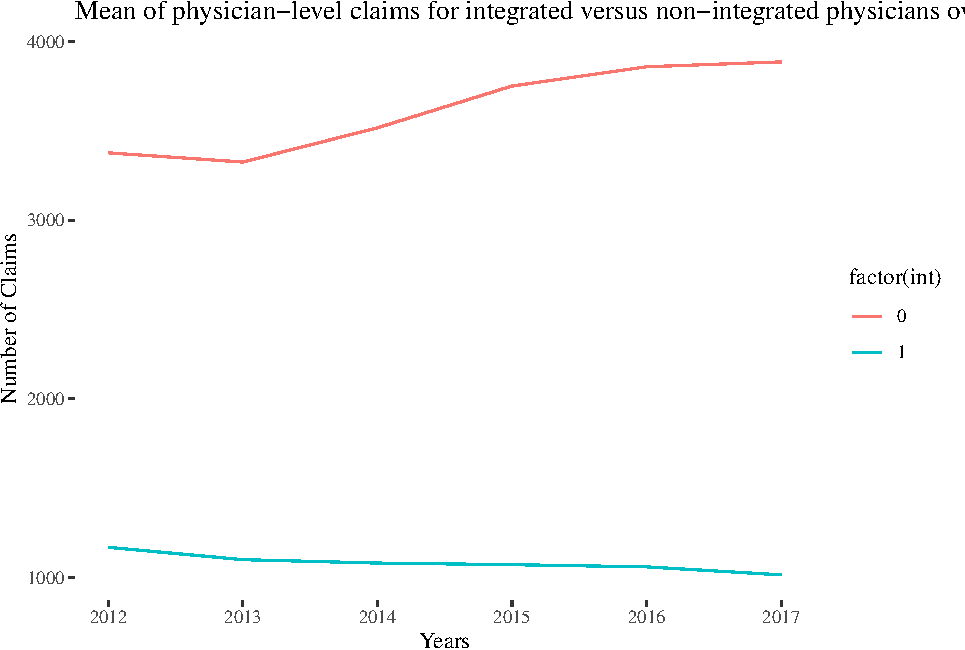
\includegraphics{Report2_files/figure-latex/Q2, -1.pdf}

We see that after the price shock implementation the total number of
claims increased for unintegrated physicians, whereas for the integrated
physicians we so not observe a change in the trend.

\begin{enumerate}
\def\labelenumi{\arabic{enumi}.}
\setcounter{enumi}{2}
\tightlist
\item
  Estimate the relationship between integration on total physician
  claims using OLS, with the following specification: \begin{equation}
   y_{it} = \delta INT_{it} + \beta x_{it} + \gamma_{i} + \gamma_{t} + \varepsilon_{it}, 
   (\#eq:ols)
   \end{equation} where \(INT_{it}\) is defined in Equation
  @ref(eq:int), \(x_{it}\) captures time-varying physician
  characteristics, and \(\gamma_{i}\) and \(\gamma_{t}\) denote
  physician and time fixed effects. Please focus on physician's that
  weren't yet integrated as of 2012, that way we have some
  pre-integration data for everyone. Impose this restriction for the
  remaining questions. Feel free to experiment with different covariates
  in \(x_{it}\) or simply omit that term and only include the fixed
  effects.
\end{enumerate}

\begingroup
\centering
\begin{tabular}{lc}
   \toprule
                                      & log\_y\\   
                                      & (1)\\  
   \midrule 
   average\_submitted\_chrg\_amt      & $1.04\times 10^{-5}$$^{***}$\\    
                                      & ($7.89\times 10^{-7}$)\\    
   average\_medicare\_payment\_amt    & 0.0002$^{***}$\\   
                                      & ($7.6\times 10^{-6}$)\\    
   int                                & -0.2624$^{***}$\\   
                                      & (0.0047)\\   
    \\
   Observations                       & 2,565,310\\  
   R$^2$                              & 0.91054\\  
   Within R$^2$                       & 0.12193\\  
    \\
   npi fixed effects                  & $\checkmark$\\   
   Year fixed effects                 & $\checkmark$\\   
   \bottomrule
\end{tabular}
\par\endgroup

The estimation results indicate that integrated physicians submit
\(0.26\%\) less claims than the unintegrated physicians.

\begin{enumerate}
\def\labelenumi{\arabic{enumi}.}
\setcounter{enumi}{3}
\tightlist
\item
  How much should we be ``worried'' about endogeneity here? Extending
  the work of @altonji2005, @oster2019 derives the expression
  \begin{equation}
   \delta^{*} \approx \hat{\delta}_{D,x_{1}} - \rho \times \left[\hat{\delta}_{D} - \hat{\delta}_{D,x_{1}}\right] \times \frac{R_{max}^{2} - R_{D,x_{1}}^{2}}{R_{D,x_{1}}^{2} - R_{D}^{2}} \xrightarrow{p} \delta,
   (\#eq:oster)
   \end{equation} where \(x_{1}\) captures our observable covariates (or
  fixed effects in our case); \(\delta\) denotes the treatment effect of
  interest; \(\hat{\delta}_{D,x_{1}}\) denotes the coefficient on \(D\)
  from a regression of \(y\) on \(D\) and \(x_{1}\); \(R_{D,x_{1}}^{2}\)
  denotes the \(R^{2}\) from that regression; \(\hat{\delta}_{D}\)
  denotes the coefficient on \(D\) from a regression of \(y\) on \(D\)
  only; \(R_{D}^{2}\) reflects the \(R^{2}\) from that regression;
  \(R_{max}^{2}\) denotes an unobserved ``maximum'' \(R^{2}\) from a
  regression of \(y\) on \(D\), observed covariates \(x_{1}\), and some
  unobserved covariates \(x_{2}\); and \(\rho\) denotes the degree of
  selection on observed variables relative to unobserved variables. One
  approach that Oster suggests is to consider a range of \(R^{2}_{max}\)
  and \(\rho\) to bound the estimated treatment effect, where the bounds
  are given by
  \(\left[ \hat{\delta}_{D,x_{1}}, \delta^{*}(R^{2}_{max}, \rho) \right]\).
  Construct these bounds based on all combinations of
  \(\rho \in (0, .5, 1, 1.5, 2)\) and
  \(R_{max}^{2} \in (0.5, 0.6, 0.7, 0.8, 0.9, 1)\) and present your
  results in a table. What do your results say about the extent to which
  selection on observables could be problematic here? Hint: you can also
  look into \texttt{psacalc} in \texttt{Stata} or \texttt{robomit} in
  \texttt{R} for implementation of @oster2019 in \texttt{Stata} or
  \texttt{R}, respectively.
\end{enumerate}

\% latex table generated in R 4.2.1 by xtable 1.8-4 package \% Fri Oct
14 21:17:24 2022

\begin{table}[ht]
\centering
\begin{tabular}{ccc}
  \hline
 & \$R\_\{max\}\verb|^|2=0.9\$ & \$R\_\{max\}\verb|^|2=1\$ \\ 
  \hline
\$ho=0\$ & [-0.36,-0.36] & [-0.36,-0.36] \\ 
  \$ho=0.5\$ & [-0.36,-0.36] & [-0.36,-0.33] \\ 
  \$ho=1\$ & [-0.36,-0.36] & [-0.36,-0.31] \\ 
  \$ho=1.5\$ & [-0.36,-0.36] & [-0.36,-0.29] \\ 
  \$ho=2\$ & [-0.36,-0.36] & [-0.36,-0.26] \\ 
   \hline
\end{tabular}
\caption{Altonji, Elder, and Taber (2005)} 
\end{table}

used (Mb) gc trigger (Mb) max used (Mb) Ncells 3973315 212.2 10819183
577.9 9330216 498.3 Vcells 48024996 366.5 145553002 1110.5 145436358
1109.6

From the regression presented in table 1 we see that the \(R^2_{D,x_1}\)
was 0.91. Thus, we omit \(R^2_{max} \leq 0.9\). In all the simulations
the bounds remain negative. Thus

\begin{enumerate}
\def\labelenumi{\arabic{enumi}.}
\setcounter{enumi}{4}
\tightlist
\item
  Construct the change in Medicare payments achievable for an integrated
  versus non-integrated physician practice due to the 2010 update to the
  physician fee schedule, \(\Delta P_{it}\). Use this as an instrument
  for \(INT_{it}\) in a 2SLS estimator following the same specification
  as in Equation @ref(eq:ols). Present your results along with those of
  your ``first stage'' and ``reduced form''.
\end{enumerate}

Yes, the idea of summing a ratio is a bit odd. But it's easier to think
of the instrument as the product of baseline (pre-shock) practice size
and the average relative revenue change due to the price shock. In that
context, the sum of the ratio is really just an interaction term that
incorporates information on the price shock magnitude and baseline
practice size. Each of these things alone are poor instruments, but
together for the practice it reflects a ``better'' instrument.

\begingroup
\centering
\begin{tabular}{lccc}
   \toprule
    & int & \multicolumn{2}{c}{log\_y}\\
                                      & (1)                           & (2)                            & (3)\\  
   \midrule 
   practice\_rev\_change              & $1.33\times 10^{-5}$$^{***}$  & $-4.29\times 10^{-5}$$^{***}$  &   \\   
                                      & ($6.76\times 10^{-7}$)        & ($1.57\times 10^{-6}$)         &   \\   
   average\_submitted\_chrg\_amt      &                               & $1.02\times 10^{-5}$$^{***}$   & $1.02\times 10^{-5}$$^{***}$\\    
                                      &                               & ($9.29\times 10^{-7}$)         & ($9.29\times 10^{-7}$)\\    
   average\_medicare\_payment\_amt    &                               & 0.0003$^{***}$                 & 0.0003$^{***}$\\   
                                      &                               & ($8.83\times 10^{-6}$)         & ($8.83\times 10^{-6}$)\\    
   INThat                             &                               &                                & -3.233$^{***}$\\   
                                      &                               &                                & (0.1184)\\   
    \\
   Observations                       & 2,176,278                     & 2,176,278                      & 2,176,278\\  
   R$^2$                              & 0.89170                       & 0.92032                        & 0.92032\\  
   Within R$^2$                       & 0.00235                       & 0.12169                        & 0.12169\\  
    \\
   npi fixed effects                  & $\checkmark$                  & $\checkmark$                   & $\checkmark$\\   
   Year fixed effects                 & $\checkmark$                  & $\checkmark$                   & $\checkmark$\\   
   \bottomrule
\end{tabular}
\par\endgroup

Endogeneity can be a threat for identification if the number of claims
affect the decision to merge. Thus, table4 presents the results of the
two stage least squares. We observe how the estimates decrease,
indicating that the number of claims for unintegrated physicians further
decline given the price shock.

\begin{enumerate}
\def\labelenumi{\arabic{enumi}.}
\setcounter{enumi}{5}
\tightlist
\item
  Assess the ``need'' for IV by implementing a Durbin-Wu-Hausman test
  with an augmented regression. Do this by first estimating the
  regression,
  \(INT_{it} = \lambda \Delta P_{it} + \beta x_{it} + \gamma_{i} + \gamma_{t} + \varepsilon_{it}\),
  take the residual \(\hat{\nu} = INT_{it} - \hat{INT}_{it}\), and run
  the regression
  \[y_{it} = \delta INT_{it} + \beta x_{it} + \gamma_{i} + \gamma_{t} + \kappa \hat{\nu} + \varepsilon_{it}.\]
  Discuss your results for \(\hat{\kappa}\).
\end{enumerate}

\begingroup
\centering
\begin{tabular}{lc}
   \toprule
                                      & log\_y\\   
                                      & (1)\\  
   \midrule 
   int                                & -3.444$^{***}$\\   
                                      & (0.1253)\\   
   average\_submitted\_chrg\_amt      & $1.3\times 10^{-5}$$^{***}$\\    
                                      & ($9.31\times 10^{-7}$)\\    
   average\_medicare\_payment\_amt    & 0.0002$^{***}$\\   
                                      & ($9.66\times 10^{-6}$)\\    
   v\_hat                             & 3.204$^{***}$\\   
                                      & (0.1251)\\   
    \\
   Observations                       & 2,176,278\\  
   R$^2$                              & 0.92079\\  
   Within R$^2$                       & 0.12692\\  
    \\
   npi fixed effects                  & $\checkmark$\\   
   Year fixed effects                 & $\checkmark$\\   
   \bottomrule
\end{tabular}
\par\endgroup

From the Durbin-Wu-Hausman test with an augmented regression we see how
\(\hat{v}\), the residuals, is significant which implies that there was
a systematic component in the error that has not been taken care of and
this is also driving the treatment effect. As such, this results might
be bias.

\begin{enumerate}
\def\labelenumi{\arabic{enumi}.}
\setcounter{enumi}{6}
\tightlist
\item
  Now let's pay attention to potential issues of weak instruments. As we
  discussed in class, one issue with weak instruments is that our
  typical critical values (say, 1.96 for a 95\% confidence interval)
  from the equation of interest (sometimes called the structural
  equation) are too low in the presence of a weak first-stage. These
  issues are presented very clearly and more formally in the Andrews,
  Stock, and Sun (2019) survey article. For this question, you will
  consider two forms of inference in the presence of weak instruments:
\end{enumerate}

\begin{itemize}
\tightlist
\item
  Present the results of a test of the null, \(H_{0}: \delta=0\), using
  the Anderson-Rubin Wald statistic. Do your conclusions from this test
  differ from a traditional t-test following 2SLS estimation of Equation
  @ref(eq:ols)?
\item
  Going back to your 2SLS results\ldots inflate your 2SLS standard
  errors to form the \(tF\) adjusted standard error, following Table 3
  in Lee et al.~(2021). Repeat the test of the null,
  \(H_{0}: \delta=0\), using standard critical values and the \(tF\)
  adjusted standard error.
\end{itemize}

{[}1{]} ``First stage F is 4013'' \% latex table generated in R 4.2.1 by
xtable 1.8-4 package \% Fri Oct 14 21:32:46 2022

\begin{table}[ht]
\centering
\begin{tabular}{ccc}
  \hline
 & lower & upper \\ 
  \hline
Anderson-Rubin & -4.11 & -3.84 \\ 
  Lee & -4.07 & -3.87 \\ 
   \hline
\end{tabular}
\caption{Confidence intervals} 
\label{tab:ci}
\end{table}

We do not see evidence of weak instruments as presented in the table.

\begin{enumerate}
\def\labelenumi{\arabic{enumi}.}
\setcounter{enumi}{7}
\tightlist
\item
  Following the Borusyak and Hull (2021) working paper (BH), we can
  consider our instrument as a function of some exogenous policy shocks
  and some possibly endogenous physician characteristics,
  \(\Delta P_{it}=f\left(g_{pt}; z_{ipt}\right)\), where \(g_{pt}\)
  captures overall payment shocks for procedure \(p\) at time \(t\), and
  \(z_{ip}\) denotes a physician's quantity of different procedures at
  baseline. We can implement the BH re-centering approach as follows:
\end{enumerate}

\begin{itemize}
\tightlist
\item
  Consider hypothetical price changes over a set of possible
  counterfactuals by assuming that the counterfactuals consist of
  different allocations of the observed relative price changes. For
  example, take the vector of all relative price changes, reallocate
  this vector randomly, and assign new hypothetical relative price
  changes. Do this 100 times. This isn't ``all'' possible
  counterfactuals by any means, but it will be fine for our purposes.
\item
  Construct the expected revenue change over all possible realizations
  from previously,
  \(\mu_{it} = E [\Delta P_{it}]= \sum_{s=1}^{100} \sum_{p} g_{pt}^{s} z_{ip}\).
\item
  Re-estimate Equation @ref(eq:ols) by 2SLS when instrumenting for
  \(INT_{it}\) with
  \(\tilde{\Delta} P_{it} = \Delta P_{it} - \mu_{it}\). Intuitively,
  this re-centering should isolate variation in the instrument that is
  only due to the policy and remove variation in our instrument that is
  due to physician practice styles (the latter of which is not a great
  instrument).
\end{itemize}

\begin{enumerate}
\def\labelenumi{\arabic{enumi}.}
\setcounter{enumi}{8}
\tightlist
\item
  Discuss your findings and compare estimates from different estimators.
\end{enumerate}

After all of the analysis and sensitivity tests we can see how the
integration to the hospital had a negative effect on the number of
claims physician made.

\begin{enumerate}
\def\labelenumi{\arabic{enumi}.}
\setcounter{enumi}{9}
\tightlist
\item
  Reflect on this assignment. What did you find most challenging? What
  did you find most surprising?
\end{enumerate}

These empirical assignments are a good opportunity to polish the work
flow needed to advance our own research. I enjoyed them all so far. I
found challenging working with Rmarkdown for the PDF.

\end{document}
